\section{Basic comparison proofs}\label{app:basic}
\paragraph{Notation.} All matrix norms without a subscript are Euclidean operator norms, except $\norm{\cdot}_F$ and $\norm{\cdot}_*$. Risk is one half of the stated quadratic form. The budget variable is $B$, while $d=(1-\cos\phi)/2$ is the slow eigenvalue of the balanced, unregularized mixture. A second moment need not be a centered covariance.

\begin{proof}[Proof of Proposition~\ref{prop:obstructions}]
If $G_A$ and $G_B$ commute, all their convex combinations commute. A product of exponentials is the exponential of their sum. The same identity holds for measurable schedules by simultaneous diagonalization and solving each scalar equation. Its effective mixture weight is $B^{-1}\int_0^B p(t)\,dt$ for $B>0$; the zero-budget statement is immediate.

For two phases let $X=b_1G_1$, $Y=b_2G_2$, $\Phi=e^{-Y}e^{-X}$, and $\Psi=e^{-(X+Y)}$. Cyclicity of trace gives
\[
 \norm{\Phi}_F^2=\tr(e^{-2X}e^{-2Y}).
\]
Golden--Thompson, applied to the symmetric matrices $-2X$ and $-2Y$, gives $\norm\Phi_F^2\ge\tr(e^{-2(X+Y)})=\norm\Psi_F^2$. The exponent $X+Y$ equals $BG(\bar p)$, with $\bar p=(b_1p_1+b_2p_2)/B$. Thus $\Psi$ is a feasible static comparator. Since static schedules belong to the two-phase class, their optimized risks coincide in the isotropic setting.

For positive definite $S,Q$, denote their smallest and largest eigenvalues by $s_-,s_+,q_-,q_+$. For every matrix $M$,
\[
 \tfrac12q_-s_-\norm M_F^2\le\tfrac12\tr(QMSM^\top)
 \le\tfrac12q_+s_+\norm M_F^2.
\]
Applying the upper bound to the exposure-matched static transition and the lower bound to the curriculum gives
$\R(\Psi)\le\kappa(Q)\kappa(S)\R(\Phi)$.
The optimal static risk is at most $\R(\Psi)$ for each curriculum. Taking the infimum over two-phase curricula proves the ratio bound. No product inequality with three or more independent exponents is used.
\end{proof}

\section{Exact static optimum and preparation formula}\label{app:exact}
\begin{lemma}[Common-diagonal static benchmark]\label{lem:diagonal}
Suppose symmetric generators $G_i$ have the same diagonal $(\gamma_1,\ldots,\gamma_D)$ in an orthonormal basis $(u_j)$. Suppose their convex hull contains $G_0=\sum_j\gamma_ju_ju_j^\top$, and $S=\sum_j s_ju_ju_j^\top$ with $s_j\ge0$. For $Q=I$, $G_0$ globally minimizes static risk at every $B\ge0$, with value $\frac12\sum_js_je^{-2B\gamma_j}$.
\end{lemma}
\begin{proof}
For a static generator $G$ with eigenpairs $(\lambda_k,z_k)$,
\[
 u_j^\top e^{-2BG}u_j=\sum_k (u_j^\top z_k)^2e^{-2B\lambda_k}
 \ge \exp\left(-2B\sum_k(u_j^\top z_k)^2\lambda_k\right)
 =e^{-2B\gamma_j}.
\]
The weights are nonnegative and sum to one. The inequality is scalar Jensen for the convex function $x\mapsto e^{-2Bx}$. Summing against $s_j/2$ gives the lower bound. The diagonal generator $G_0$ attains it. This is a direct spectral Jensen consequence; operator convexity of the exponential is neither assumed nor needed.
\end{proof}

\begin{proof}[Proof of Theorem~\ref{thm:static}]
In the $(u,v)$ basis, $G(p)-\rho I$ has the form
\begin{equation}
 \begin{pmatrix}a&z(p)\\z(p)&d\end{pmatrix},\qquad
 z(p)=(1-2p)\sqrt{ad}.\label{eq:bisector_matrix}
\end{equation}
Indeed $u^\top v_A=u^\top v_B=\sqrt a$, whereas $v^\top v_A=-\sqrt d$ and $v^\top v_B=\sqrt d$. The diagonal is independent of $p$, and the off-diagonal vanishes at $p=1/2$. Apply Lemma~\ref{lem:diagonal} with masses $1,\eps$.
\end{proof}

\begin{proof}[Proof of the formula in Theorem~\ref{thm:prep}]
The common ridge commutes with all terms, so every transition is multiplied by $e^{-\rho B}$. It suffices to compute at $\rho=0$. In the original source basis, $u=(\sqrt a,\sqrt d)^\top$ and $v=(-\sqrt d,\sqrt a)^\top$. Since $e^{-\tau}=c/(1+c)=c/(2a)$,
\[
 e^{-\tau v_Av_A^\top}u
 =\begin{pmatrix}c/(2\sqrt a)\\\sqrt d\end{pmatrix}
 =\frac{v_B}{2\sqrt a}.
\]
The identity uses $\sin\phi=2\sqrt{ad}$. Thus the squared norm after the second phase is
\[
 \norm{e^{-(B-\tau)v_Bv_B^\top}e^{-\tau v_Av_A^\top}u}^2
 =\frac{e^{-2(B-\tau)}}{4a}=\frac{a}{c^2}e^{-2B}=A_\phi e^{-2B}.
\]
For the orthogonal vector, define $w=e^{-\tau v_Av_A^\top}v=(-c\sqrt d/(2a),\sqrt a)^\top$ and $v_B^\perp=(-\sin\phi,\cos\phi)^\top$. Direct inner products give
\[
 (v_B^\top w)^2=\frac{d(1+2c)^2}{(1+c)^2},\qquad
 ((v_B^\perp)^\top w)^2=\frac{c^2}{a}=F_\phi.
\]
The parallel component is multiplied by $e^{-2(B-\tau)}$ and the perpendicular component is unchanged. Therefore its final squared norm is $D_\phi e^{-2B}+F_\phi$. Weighting the two initial components by $1$ and $\eps$, dividing by two, and restoring $e^{-2\rho B}$ proves \eqref{eq:prep}.
\end{proof}

\begin{proof}[Proof of the rate and work claims]
At $\eps=0$, dividing \eqref{eq:static} by \eqref{eq:prep} gives $F_\phi e^{2(1-a)B}=F_\phi e^{2dB}$. Strict improvement is equivalent to $2dB>\log A_\phi$ whenever the preparation schedule is feasible.

For every admissible allocation, $G(p(t))\preceq(1+\rho)I$. The scalar energy derivative satisfies
\[
 \frac{d}{dt}\norm{e(t)}^2=-2e(t)^\top G(p(t))e(t)
 \ge-2(1+\rho)\norm{e(t)}^2.
\]
Integration gives $\norm{e(B)}^2\ge e^{-2(1+\rho)B}\norm{e(0)}^2$. The initial vector $u$ has unit norm. This proves the lower bound for arbitrary measurable schedules; the explicit schedule supplies the upper bound. The bounds imply the same exponential rate for $\Rt$ and $\Ra$.

Solving the two explicit risk formulas for their first crossing of a sufficiently small $\ell$ gives \eqref{eq:work}. The preparation crossing eventually exceeds $\tau$. For the optimal arbitrary schedule, the lower and upper rate bounds bracket the required work between $\log(1/(2\ell))/(2(1+\rho))$ and $\log(A_\phi/(2\ell))/(2(1+\rho))$. Their difference is constant in $\ell$, so they give the same limiting static-to-curriculum work ratio.
\end{proof}

\section{Uncertainty thresholds, rate obstruction, and peak law}\label{app:uncertainty}
\begin{proof}[Proof of Theorem~\ref{thm:threshold}]
Subtracting the two exact formulas yields
\[
 2e^{2\rho B}(\Rs-\Rp)=N(B)-\eps K(B),\qquad
 K(B)=F_\phi+D_\phi e^{-2B}-e^{-2dB}.
\]
At $\eps=1$, Proposition~\ref{prop:obstructions} implies $N(B)-K(B)\le0$, since the preparation curriculum is a two-phase schedule and the balanced static mixture is optimal. If $N(B)>0$, it follows that $K(B)\ge N(B)>0$, and strict improvement is exactly $\eps<N(B)/K(B)$. This threshold is at most one. As $B\to\infty$, $N(B)\sim e^{-2aB}$ and $K(B)\to F_\phi>0$, proving the asymptotic expression. If $N(B)\le0$, the difference is nonpositive both at $\eps=0$ and at $\eps=1$. Affinity in $\eps$ proves nonpositivity throughout $[0,1]$. No assertion for $\eps>1$ is required for this threshold statement.
\end{proof}

\begin{lemma}[Slow-eigenvector cone]\label{lem:cone}
For all $p\in[0,1]$, the smaller eigenvalue of $G(p)$ in \eqref{eq:family} is at most $\rho+d$. Its unit slow eigenvector can be chosen to make angle at most $\phi/2$ with $v$, and slow eigenvectors for any two mixtures have squared inner product at least $c^2$.
\end{lemma}
\begin{proof}
In \eqref{eq:bisector_matrix}, $a-d=c>0$ and $|z(p)|\le\sqrt{ad}=\sin\phi/2$. The smaller eigenvalue is
\[
 \mu_-(p)=\rho+\frac{1-\sqrt{c^2+4z(p)^2}}{2}\le\rho+\frac{1-c}{2}=\rho+d.
\]
Diagonalization rotates the principal axes by an angle $\psi$ satisfying $|\tan(2\psi)|=2|z|/c\le\tan\phi$, with $|2\psi|<\pi/2$. Hence $|\psi|\le\phi/2$. The slow axes lie in an angular cone of width $\phi<\pi/2$, and consistently oriented unit vectors have inner product at least $\cos\phi=c$.
\end{proof}

\begin{proof}[Proof of Theorem~\ref{thm:fullrank}]
Let phase generators $G_1,G_2$ have orthonormal eigenvectors $w_{1,k},w_{2,l}$ and eigenvalues $\mu_{1,k},\mu_{2,l}$. For $\Phi=e^{-b_2G_2}e^{-b_1G_1}$, expand the trace as
\begin{equation}
 \norm\Phi_F^2=\sum_{k,l}
 e^{-2b_1\mu_{1,k}-2b_2\mu_{2,l}}
 |w_{1,k}^\top w_{2,l}|^2.\label{eq:nonnegative_expansion}
\end{equation}
Every term is nonnegative. Keep only the slow--slow term and apply Lemma~\ref{lem:cone} to obtain
$\norm\Phi_F^2\ge c^2e^{-2(\rho+d)(b_1+b_2)}$.
For $0<\eps\le1$, $S_\eps\succeq\eps I$, so $\R(\Phi)\ge\eps\norm\Phi_F^2/2$. This proves the uniform lower bound over all two-phase durations and mixture weights. The upper bound follows from the exact static formula and $a>d$. Taking logarithms and dividing by $-2B$ proves the rate for fixed positive $\eps$. The $\eps=0$ statement follows from Theorem~\ref{thm:prep}. The constants in the positive-$\eps$ lower bound vanish as $\eps\downarrow0$, which is why these limits do not commute.
\end{proof}

\begin{proposition}[Arbitrary-stage volume obstruction]\label{prop:volume}
For \eqref{eq:family}, $\eps>0$, and every measurable schedule,
\begin{equation}
 \R(\pi)\ge\sqrt\eps\,e^{-(1+2\rho)B}.
\end{equation}
\end{proposition}
\begin{proof}
The trace of every generator is $1+2\rho$. Liouville's determinant formula gives $\det\Phi_\pi=e^{-(1+2\rho)B}$. The two eigenvalues of $\Phi_\pi S_\eps\Phi_\pi^\top$ are positive, with product $\eps e^{-2(1+2\rho)B}$. Arithmetic--geometric mean bounds their sum below by twice the square root of this product. Dividing by two proves the result. This does not imply the sharper two-phase exponent $\rho+d$ for arbitrary schedules.
\end{proof}

\begin{proof}[Proof of Corollary~\ref{cor:peak}]
Put $x=e^{-2B}$, $A_\eps=A_\phi+\eps D_\phi$, and suppress the fixed angle subscript on $F$. The ratio is
\[
 \frac{x^a+\eps x^d}{A_\eps x+\eps F},\qquad
 0<x\le e^{-2\tau},\quad a+d=1.
\]
For $f(x)=x^a/(A_\eps x+\eps F)$, differentiation shows its unique unrestricted maximum is at
\[
 x_*=\frac{a\eps F}{d A_\eps},\qquad
 f(x_*)=a^ad^dA_\eps^{-a}F^{-d}\eps^{-d}.
\]
For sufficiently small $\eps$, $x_*$ lies in the admissible interval. The second summand $g(x)=\eps x^d/(A_\eps x+\eps F)$ is uniformly $O(\eps^d)$: substitute $x=\eps t$ and use boundedness of $t^d/(A_\eps t+F)$ on $t>0$, uniformly as $\eps\downarrow0$. Consequently the maximum of $f+g$ differs from the maximum of $f$ by at most $O(\eps^d)$. Since $F=A_\phi^{-1}$ and $a-d=c$, the leading constant converges to $a^ad^dA_\phi^{-a+d}=a^ad^dA_\phi^{-c}$.
\end{proof}

\begin{figure}[t]
\centering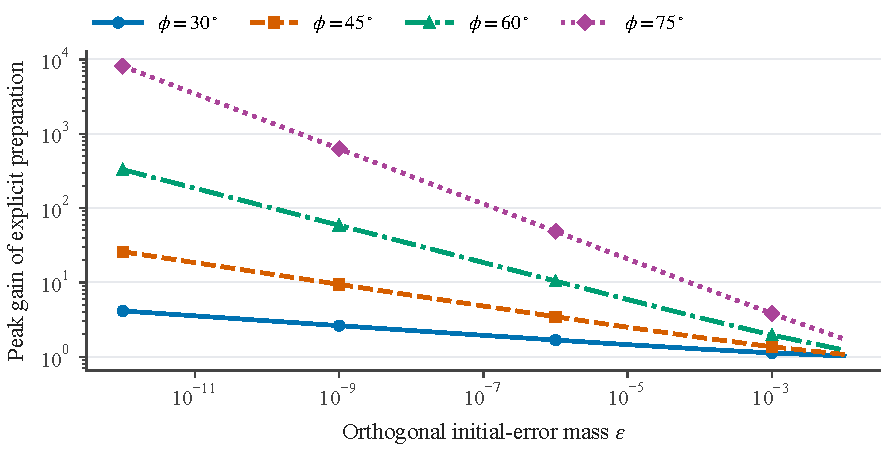
\includegraphics[width=.92\linewidth]{figures/peak_gain.pdf}
\caption{The peak preparation gain grows as orthogonal uncertainty decreases. The exponent is $d=(1-\cos\phi)/2$, so the gain can increase slowly when the source directions are close. The plotted maxima are one-dimensional numerical evaluations of the exact formulas; Corollary~\ref{cor:peak} is analytic.}\label{fig:peak}
\end{figure}

\section{Spectral and capacity-work proof}\label{app:spectral}
\begin{lemma}[Power-law exponential tail sum]\label{lem:tail}
For fixed $\alpha,\beta,k>0$,
\[
 \sum_{j\ge1}j^{-1-\beta}e^{-kBj^{-\alpha}}\asymp B^{-\beta/\alpha}
 \quad(B\ge1).
\]
The same conclusion holds when the weights and scales are comparable, with fixed positive constants, to $j^{-1-\beta}$ and $j^{-\alpha}$.
\end{lemma}
\begin{proof}
Write $J_B=\lceil B^{1/\alpha}\rceil$. For $j\ge J_B$, the exponential is bounded below by a positive constant depending only on $k,\alpha$, and the tail sum is comparable to $J_B^{-\beta}$. This proves the lower bound. For the upper bound, the same tail is at most a constant times $J_B^{-\beta}$. Partition $1\le j<J_B$ into dyadic bands with $j$ between $2^{-l-1}J_B$ and $2^{-l}J_B$, omitting empty bands. The total weight of a band is at most a constant times $J_B^{-\beta}2^{(l+1)\beta}$, while its exponential is at most $\exp(-k'2^{l\alpha})$ for a fixed $k'>0$. The series over bands converges independently of $B$, because exponential decay in $2^{l\alpha}$ dominates the geometric factor. Comparability changes only constants.
\end{proof}

\begin{proof}[Proof of Theorem~\ref{thm:spectral}]
For every trained block and every schedule, the energy differential inequality gives
\[
 \norm{e_j(B)}^2\ge e^{-2L\lambda_jB}\norm{e_j(0)}^2.
\]
Expectation gives the same bound with initial mass $w_j$. The proposed static mixture gives the upper bound $\E\norm{e_j(B)}^2\le e^{-2m\lambda_jB}w_j$. Hence
\[
 \tfrac12\sum_{j\le J}w_je^{-2L\lambda_jB}+\tfrac12\sum_{j>J}w_j
 \le\R^*(B,J)
 \le\tfrac12\sum_{j\le J}w_je^{-2m\lambda_jB}+\tfrac12\sum_{j>J}w_j.
\]
The lower expression is at least the full exponential sum, because each untrained tail term is at least its exponentially damped version. It is also at least the untrained mass. Lemma~\ref{lem:tail} and $\sum_{j>J}w_j\asymp J^{-\beta}$ therefore give a constant times $B^{-\beta/\alpha}+J^{-\beta}$ as a lower bound, using $\max(x,y)\ge(x+y)/2$. The upper expression is at most the full exponential sum plus the tail, proving the corresponding upper bound. In particular, no interchange of an unbounded number of blocks with a block-specific schedule is involved.

For total work $JB\le C$, the lower bound gives, up to constants,
\[
 B^{-\beta/\alpha}+J^{-\beta}
 \ge B^{-\beta/\alpha}+(B/C)^\beta.
\]
The two terms balance at $B\asymp C^{\alpha/(\alpha+1)}$. Either side of that scale is bounded below by a constant times $C^{-\beta/(\alpha+1)}$. Taking $J$ to be an integer within a constant factor of $C^{1/(\alpha+1)}$ and using the common static mixture gives the matching upper bound. The cost counts a fixed capacity during training; it is not a result about dynamically activating features.
\end{proof}

\section{Perturbation, discretization, and statistical bounds}\label{app:certificate}
\begin{lemma}[Uniform transition perturbation]\label{lem:duhamel}
Suppose two time-dependent symmetric PSD generators differ in operator norm by at most $\delta_G$ almost everywhere on $[0,T]$. Their transitions satisfy
$\norm{\Phi(T)-\widehat\Phi(T)}\le\min\{2,T\delta_G\}$.
\end{lemma}
\begin{proof}
All subinterval transitions are contractions. Variation of constants gives
\[
 \Phi(T)-\widehat\Phi(T)=
 -\int_0^T\Phi(T,s)(G(s)-\widehat G(s))\widehat\Phi(s,0)\,ds.
\]
The integral norm is at most $T\delta_G$. The triangle inequality and contraction bounds also give two. For source estimates with per-source errors bounded by $\delta_G$, every common convex allocation has an error at most $\delta_G$. Thus this result is simultaneous over schedules.
\end{proof}

\begin{proof}[Uniform risk and oracle bounds]
For $Q=I$, split the risk difference by first replacing $S$ by $\widehat S$ and then replacing $\Phi$ by $\widehat\Phi$. The covariance term has absolute value at most $\delta_S/2$, since $\norm{\Phi^\top\Phi}\le1$. If $\eta_\Phi=\norm{\Phi-\widehat\Phi}$, then
\[
 \norm{\Phi^\top\Phi-\widehat\Phi^\top\widehat\Phi}
 \le(\norm\Phi+\norm{\widehat\Phi})\eta_\Phi\le2\eta_\Phi.
\]
Because $\widehat S\succeq0$, the remaining risk difference is at most $\tr(\widehat S)\eta_\Phi$. Apply Lemma~\ref{lem:duhamel} to obtain \eqref{eq:uniform}.

If an empirical library minimizer has tolerance $\eta$, compare its true risk to its estimated risk, use empirical optimality, and compare the selected reference's estimated risk to its true risk. The two estimation differences contribute at most $2r_T$, proving the oracle inequality. An infimum can replace an attained optimum by an arbitrarily small additional tolerance. All terms use the same post-pilot budget $T$.
\end{proof}

\paragraph{Robustness of a strict comparison.}
For a nominal schedule with gap $\Delta=\R_{\mathrm{stat},0}^*(B)-\R_0(\pi)>0$, a uniform radius $r_B$ for both schedule and static risks gives
$\Rs(B)-\R(\pi)\ge\Delta-2r_B$.
Thus every positive nominal gap has a nonempty neighborhood of source/second-moment perturbations in which the comparison persists. This is an absolute-risk statement. Since the gap can be exponentially small, it is not a uniform large-budget robustness guarantee. The experiment records this conservative certificate separately from actual perturbed gains.

\begin{lemma}[Euler-to-flow bound at a specified schedule]\label{lem:euler}
Suppose every step uses a symmetric PSD generator with norm at most $L$, the common step size is $\eta$ with $\eta L\le1$, and there are $K$ steps, with total work $B=K\eta$. The Euler transition product and the exact piecewise-constant flow with the same stepwise allocation differ by at most $B\eta L^2/2$ in operator norm.
\end{lemma}
\begin{proof}
For $x\in[0,1]$, $0\le e^{-x}-(1-x)\le x^2/2$. Spectral calculus therefore bounds each one-step discrepancy by $\eta^2L^2/2$. Both the Euler factor and the exponential factor have norm at most one. A telescoping product identity bounds the total discrepancy by the sum of one-step discrepancies, namely $K\eta^2L^2/2$. Rounding a phase boundary is a separate change in the schedule; the experiment compares flow and Euler using identical rounded durations.
\end{proof}

\paragraph{Gaussian observation event.}
In the direct coordinate-query model, $\widehat e-e$ has law $(\sigma/\sqrt n)Z$ with $Z\sim N(0,I_D)$. Gaussian concentration for the 1-Lipschitz Euclidean norm gives $\Pr(\norm Z\ge\E\norm Z+t)\le e^{-t^2/2}$; Jensen gives $\E\norm Z\le\sqrt D$. Choosing $t=\sqrt{2\log(1/\delta)}$ yields \eqref{eq:gaussian}. These are classical concentration tools \citep{boucheron2013}. Candidate selection does not require a union bound when all candidate risks are bounded on this same state-ball event.

\section{Uniform static envelopes and the paid gate}\label{app:envelope}
This section supplies the global lower comparator used by the pilot. It is not needed for the exact-family optimum. Consider known generators, fixed full budget $B$, and $E(p)=e^{-BG(p)}$. Partition $[0,1]$ into cells centered at $q$ with half-width $h_q$. Let $m_q$ be the minimum of the smallest eigenvalues of the two endpoint generators. Concavity of the smallest eigenvalue implies $G(p)\succeq m_q I$ throughout the cell. Duhamel's formula then gives
\begin{equation}
 \norm{E(p)-E(q)}\le\eta_q:=B\norm{G_A-G_B}h_qe^{-Bm_q}.\label{eq:cell}
\end{equation}
Both generators along the interpolation have the stated lower bound, so the two exponential factors in the integral contribute $e^{-Bm_q}$. If true and estimated source generators differ by at most $\delta_G$, one can add $\min\{2,B\delta_G\}$ to $\eta_q$ by a triangle inequality.

Write $N=\norm{\widehat e}$, $y_q=E(q)\widehat e$, $n_q=\norm{E(q)}$, and $n_q^+=\min\{1,n_q+\eta_q\}$. On the state ball $\norm{e-\widehat e}\le r$, the triangle inequality supplies the cell-wise lower bound
\begin{equation}
 L_q^{\mathrm{amp}}=\tfrac12
 \left[\norm{y_q}-n_qr-\eta_q(N+r)\right]_+^2.\label{eq:amplower}
\end{equation}
A usually sharper bound follows from convexity of $f_p(e)=\norm{E(p)e}^2/2$:
\[
 f_p(e)\ge f_p(\widehat e)-r\norm{E(p)^2\widehat e}.
\]
The first term is bounded below by $\frac12[\norm{y_q}-\eta_qN]_+^2$. To bound the gradient norm, use
\[
 (E(p)^2-E(q)^2)\widehat e
 =E(p)(E(p)-E(q))\widehat e+(E(p)-E(q))y_q.
\]
Hence a second cell-wise lower bound is
\begin{equation}
 L_q^{\mathrm{dir}}=\tfrac12[\norm{y_q}-\eta_qN]_+^2
 -r\left(\norm{E(q)y_q}+\eta_q(\norm{y_q}+n_q^+N)\right).
\end{equation}
It follows that
\begin{equation}
 L_s(B)=\max\left\{0,\min_q\max\{L_q^{\mathrm{amp}},L_q^{\mathrm{dir}}\}\right\}
 \le\inf_{p\in[0,1]}\tfrac12\norm{E(p)e}^2.\label{eq:uniformlower}
\end{equation}
The bounds cover the whole cell rather than only its center, so optimizing on a grid does not invalidate the comparator.

\paragraph{Candidate upper bound.}
For $e=\widehat e+z$ with $\norm z\le r$, expand
\[
 \tfrac12\norm{\Phi e}^2
 =\tfrac12\norm{\Phi\widehat e}^2+
 z^\top\Phi^\top\Phi\widehat e+\tfrac12z^\top\Phi^\top\Phi z.
\]
Cauchy--Schwarz proves \eqref{eq:upper}. The amplitude bound $\frac12(\norm{\Phi\widehat e}+r\norm\Phi)^2$ is also valid, and the implementation takes the smaller bound. If an estimated transition has error $\eta_\Phi$, its directional bound can be enlarged by
$\frac12\eta_\Phi(2\norm{\widehat\Phi}+\eta_\Phi)(N+r)^2$.

\paragraph{Decision and budget.}
Each candidate may have a different remaining training budget if its additional cost differs. A valid upper bound uses that actual remaining budget. The baseline lower bound always uses the full original $B$. Taking the smallest candidate upper bound is valid on the common confidence event. If it is below \eqref{eq:uniformlower}, the accepted candidate beats every full-budget static mixture. This proves Proposition~\ref{prop:accept}. A static fallback after rejection has only $T$ training work, not $B$, so a claim of unconditional no-regression would be false.

\paragraph{Numerical status.}
The real-arithmetic statements above are inequalities. The supplied implementation computes eigendecompositions in float64 and pads bounds outward by $10^{-12}$. Padding is a precaution, not a proof of every floating-point operation's rounding error. The exact comparison theorems rely on analytic formulas, independently checked with 70-digit matrix exponentials; the pilot code remains a numerical realization of a mathematical certificate. A formally machine-verified gate would require directed-rounding linear algebra or a separately proved floating-point error bound.
